% Created 2024-07-30 Tue 09:14
% Intended LaTeX compiler: pdflatex
\documentclass[11pt]{article}
\usepackage[utf8]{inputenc}
\usepackage[T1]{fontenc}
\usepackage{graphicx}
\usepackage{longtable}
\usepackage{wrapfig}
\usepackage{rotating}
\usepackage[normalem]{ulem}
\usepackage{amsmath}
\usepackage{amssymb}
\usepackage{capt-of}
\usepackage{hyperref}
\usepackage{minted}
\usepackage{xcolor}
\usepackage{hyperref}
\usepackage{tocloft}
\usepackage[margin=1in]{geometry}
\usepackage{fancyhdr}
\usepackage{fancyheadings}
\usepackage{titlepic}
\usepackage{pdfpages}
\usepackage[T1]{fontenc}
\usepackage{helvet}
\usepackage{fontawesome}
\usepackage[colorlinks=true, urlcolor=blue, linkcolor=blue]{hyperref}
\usepackage{graphicx}
\usepackage[mmddyyyy]{datetime}
\usepackage{fancyhdr}
\setlength{\parskip}{2mm}
\setlength{\parindent}{0mm}
\setcounter{secnumdepth}{3}
\setcounter{tocdepth}{3}
\usepackage{setspace}
\usepackage{wrapfig}
\hypersetup{breaklinks=true}
\usepackage{verbatim}
\usepackage{fvextra}
\usepackage{float}
\usepackage{lipsum}
\author{Hilduara Abreu}
\date{\today}
\title{PS192 Handbook}
\hypersetup{
 pdfauthor={Hilduara Abreu},
 pdftitle={PS192 Handbook},
 pdfkeywords={},
 pdfsubject={},
 pdfcreator={Emacs 29.4 (Org mode 9.6.15)}, 
 pdflang={English}}
\begin{document}

\maketitle
\tableofcontents


\section{Cover Page}
\label{sec:org018b6dc}
\begin{center}
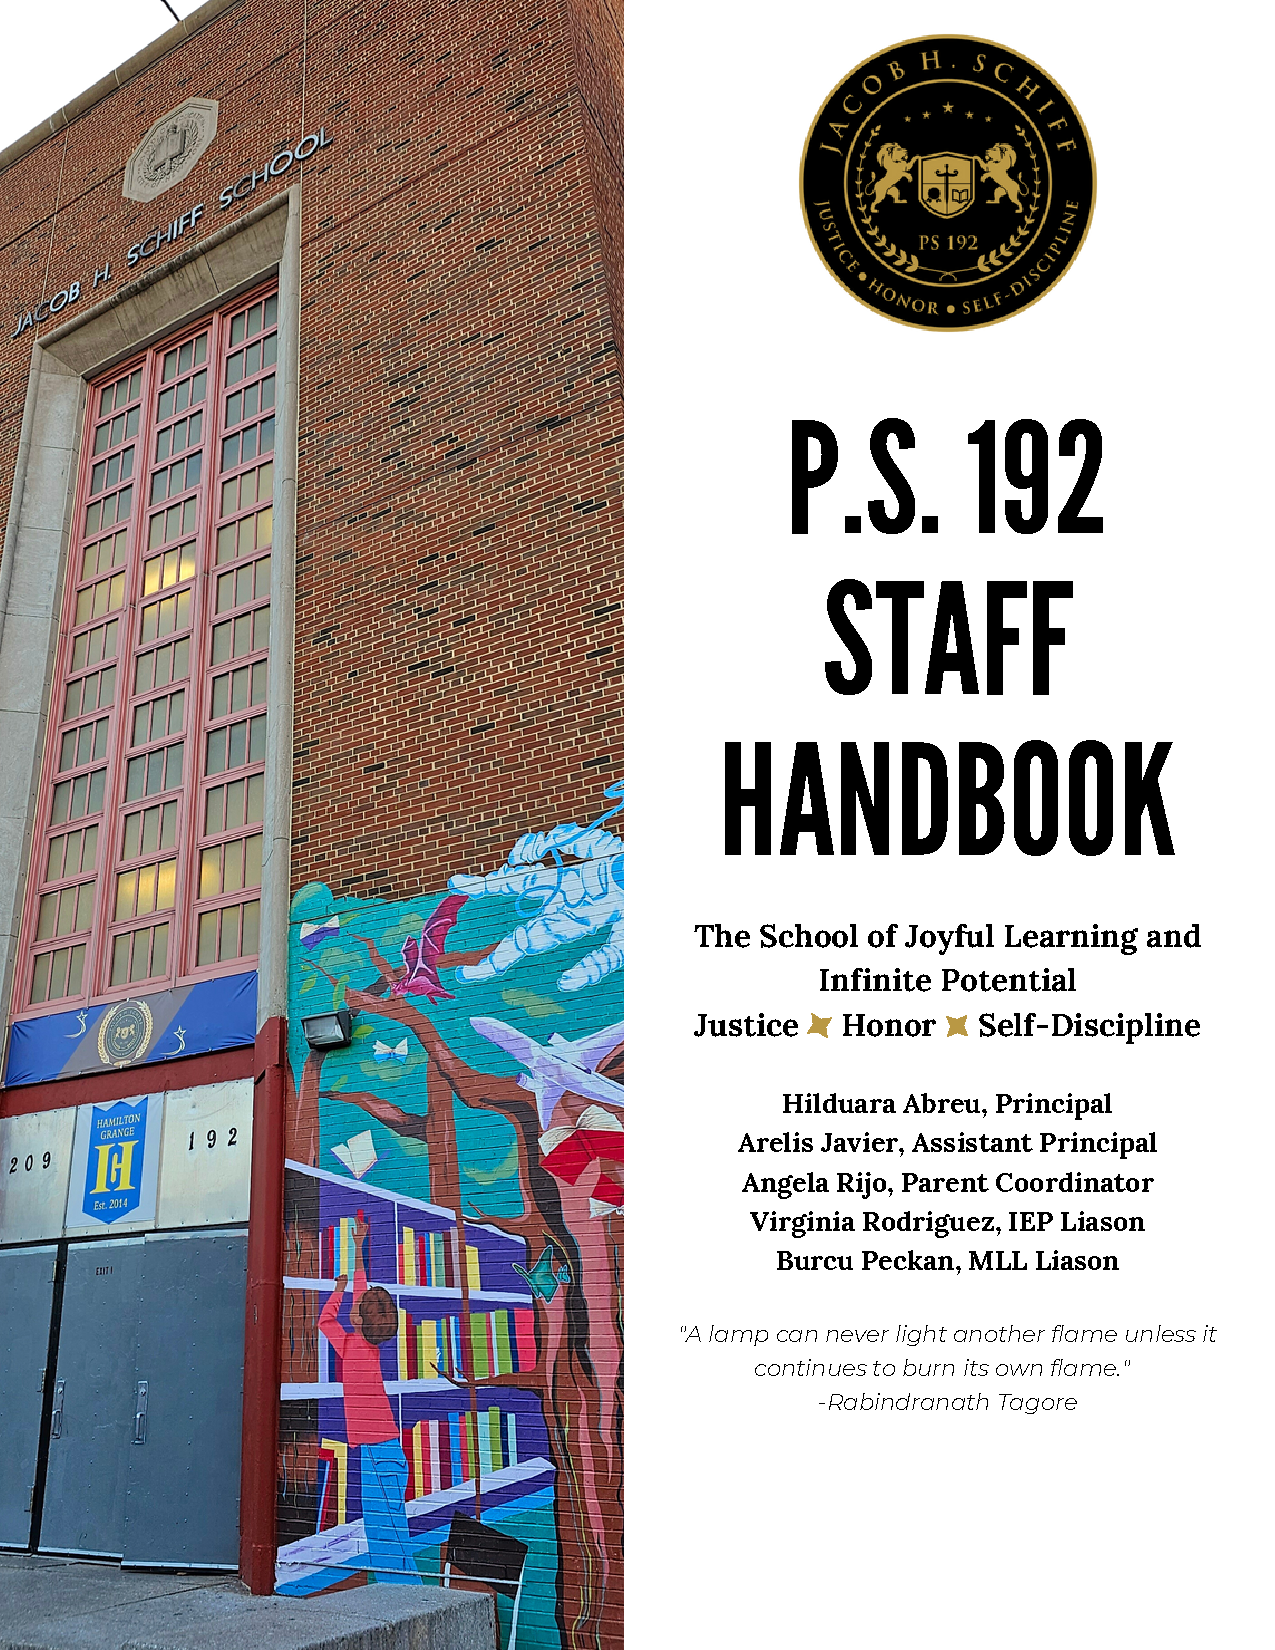
\includegraphics[width=.9\linewidth]{./handbook_front.pdf}
\end{center}

\section{Header and Footer}
\label{sec:org06e988d}
\begin{verbatim}
\pagenumbering{\fancyhf{}}
\pagestyle{headings}
\pagenumbering{arabic}
\fancyhead[L]{\textit{\rightmark}}
\fancyhead[R]{\thepage}
\fancyfoot[C]{The School of Joyful Learning!}
\pagestyle{fancy}
\renewcommand{\footrulewidth}{1px}
\end{verbatim}

\section{Table of Contents}
\label{sec:org351620b}
\tableofcontents

\% Message from the Principal
\%\%\%\%\%\%\%\%\%\%\%\%\%\%\%\%\%\%\%\%\%\%\%\%\%\%\%\%\%\%\%\%\%\%\%\%\%\%\%\%\%\%\%\%\%\%\%\%\%\%\%\%\%\%\%\%\%\%\%\%\%\%\%\%\%\%\%\%\%\%\%\%\%\%\%\%\%\%\%\%\%\%\%\%\%\%\%\%\%\%\%\%\%\%\%\%\%\%
\newpage
\section{Message From Principal Abreu}

Dear Staff:

Welcome to the 2023-2024 edition of the PS 192: Jacob H. Schiff  Faculty and Staff Handbook. It is the responsibility of each staff member to be fully acquainted with the information contained herein. This handbook is a living document and it will be updated, as necessary, throughout the year. It is meant to provide information and procedures that are important for the smooth operation of our PS 360 community. This handbook is a guide for ALL STAFF MEMBERS about the daily operation of our school. Please familiarize yourselves with your individual and school-wide responsibilities. Please do not hesitate to ask questions or get further clarification regarding any policy or procedure.

I encourage you to begin by thoroughly acquainting or re-acquainting yourself with our school’s philosophy, mission, objectives and core principles, as outlined in the School Overview. Key elements of this vision are elaborated upon throughout the handbook, along with important information about structures and policies that support our school mission and ensure the safety and success of all members of our school community.

During the upcoming school year, we will continue to strengthen and deepen our work in relation to NYCDOE and District 6 priorities, as reflected in our School Problem of Practice, priorities and CEP Goals. These areas will be central to our work as a Professional Learning Community and will be further addressed in Professional Learning sessions and Professional Planning Teams, as well as in administrative memos and guidelines, many of which can be accessed in Appendix B of this handbook.

I look forward to our continued collaboration in the year ahead.

Respectfully yours,


\includegraphics[width=0.2\textwidth]{hil_signature}

Hilduara Abreu

Principal

\textbf{The School of Joyful Learning!}

\href{https:www.ps192.org}{www.ps192.org}
$\backslash$
\end{document}
